%----------------------------------------------------------------------------------------
%    TITLE PAGE
%----------------------------------------------------------------------------------------

\title{Persistência de Dados - Parte 2}

\author{Prof. Gabriel Rodrigues Caldas de Aquino}

\institute
{
    gabrielaquino@ic.ufrj.br\\
    
    Instituto de Computação -
    Universidade Federal do Rio de Janeiro % Your institution for the title page
}
\date{03 de Junho de 2025} % Date, can be changed to a custom date

%----------------------------------------------------------------------------------------
%    PRESENTATION SLIDES
%----------------------------------------------------------------------------------------



\begin{frame}
    % Print the title page as the first slide
    \titlepage
\end{frame}

%------------------------------------------------
\section{Sobre persistência de dados}
%------------------------------------------------





\begin{frame}[fragile]{Abrindo Arquivos em Python}
    \begin{block}{Método \texttt{open()}}
        Usado para abrir um arquivo. Requer dois parâmetros principais:
\begin{verbatim}
    arquivo = open("nome_do_arquivo.txt", "modo_de_abertura")
\end{verbatim}
        
    \end{block}
    
    \begin{columns}[T]
        \begin{column}{0.5\textwidth}
            \begin{exampleblock}{Parâmetros}
                \begin{itemize}
                    \item \textbf{Nome do arquivo}: \begin{itemize}
                        \item Caminho completo ou relativo
                    \end{itemize}
                    \item \textbf{Modo de abertura}:
                    \begin{itemize}
                        \item \texttt{"r"} - Leitura 
                        \item \texttt{"w"} - Escrita 
                    \end{itemize}
                \end{itemize}
            \end{exampleblock}
        \end{column}
        
        \begin{column}{0.5\textwidth}
            \begin{alertblock}{Exemplos}
\begin{verbatim}
   
# Para escrita
arq = open("dados.txt", "w")

# Para leitura
arq = open("dados.txt", "r")

\end{verbatim}
            \end{alertblock}
        \end{column}
    \end{columns}
    
    \vspace{0.3cm}
    

\end{frame}



\begin{frame}{Modos de Abertura de Arquivo}

\centering
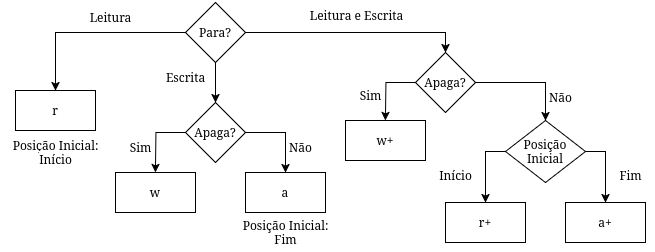
\includegraphics[width=0.8\textwidth]{Images/diagrama-modos-leitura.png}


\end{frame}


\begin{frame}[fragile]{Abrindo Arquivos}
\begin{itemize}
    \item Método read: ler dados de um arquivo que foi previamente aberto para leitura
    \item Para abrir um arquivo para leitura: 
    \begin{itemize}
        \item Precisamos dar o nome de um arquivo existente 
        \item Em seguida indicar o modo de leitura \textit{r} no momento da abertura
    \end{itemize}

\end{itemize}

\begin{block}{Abrindo o arquivo dados.txt}
\begin{verbatim}
arquivo = open("dados.txt", "r")
conteudo = arquivo.read()
print(conteudo)
arquivo.close()
\end{verbatim}
\end{block}

\end{frame}



\begin{frame}[fragile]{Lendo linha por linha}

\begin{itemize}
    \item Em arquivos com múltiplas linhas podemos usar for loop para facilitar o tratamento linha por linha
\end{itemize}
    
\begin{exampleblock}{Exemplo de leitura linha por linha}
\begin{verbatim}
arquivo="dados.txt"
arq = open(arquivo, "r")
numero_da_linha = 1
for linha in arq:
    print(f"Linha {numero_da_linha}: {linha}")
    numero_da_linha = numero_da_linha + 1
arq.close()
\end{verbatim}
\end{exampleblock}


\end{frame}



\begin{frame}[fragile]{Escrita Básica em Arquivos}
\begin{block}{Exemplo de escrita em arquivo}
\begin{verbatim}
arq = open("nomes.txt", "w")
arq.write("Gabriel, Pedro, Manoel")
arq.close()
\end{verbatim}
\end{block}

\begin{block}{Importante!}
\begin{itemize}
\item \texttt{'w'} = write (escrita)
\item Sempre feche o arquivo após escrever
\item Cada \texttt{write()} grava o conteúdo exato
\item Se o arquivo "nomes.txt" \textbf{já existe}, ele será \textbf{sobrescrito}
\end{itemize}
\end{block}
\end{frame}

\begin{frame}[fragile]{Arquivos com mais de uma linha}

\begin{block}{Leitura de Arquivos Linha por Linha}
\begin{itemize}
    \item Arquivos com múltiplas linhas contêm \texttt{\textbackslash n} escondido

\end{itemize}
\end{block}

\begin{exampleblock}{Exemplo Prático}
Pedro\textbackslash n

Antonio\textbackslash n

Maria\textbackslash n

Jose\textbackslash n
\end{exampleblock}

\end{frame}

\begin{frame}[fragile]{Pulando linha na escrita em arquivos}

\begin{block}{Código de exemplo}
\begin{verbatim}
arq = open("nomes.txt", "w")
arq.write("Gabriel\nPedro\nManoel")
arq.close()
\end{verbatim}
\end{block}



\begin{alertblock}{O que acontece?}
\begin{itemize}
\item \texttt{\textbackslash n} é o \textbf{caractere especial} para quebra de linha
\item Quando escrito no arquivo, ele:
  \begin{itemize}
  \item Finaliza a linha atual
  \item Move o cursor para a próxima linha
  \end{itemize}

\end{itemize}
\end{alertblock}


\end{frame}

